\iffalse
\chapter{2015}
\author{AI24BTECH11022}
\section{ae}
\fi

\item Choose the appropriate word/phrase, out of the four options given below, to complete the following sentence.

Apparent lifelessness \rule{1cm}{0.15mm} dormant life.\hfill(2015)
\begin{multicols}{2}
\begin{enumerate}
\item harbours
\item leads to
\item supports
\item affects
\end{enumerate}
\end{multicols}


\item Fill in the blank with the correct idiom/phrase.

That boy from the town was a \rule{1cm}{0.15mm} in the sleepy village.\hfill(2015)
\begin{multicols}{2}
\begin{enumerate}
\item dog out of herd
\item sheep from the heap
\item fish out of water
\item bird from the flock
\end{enumerate}
\end{multicols}


\item Choose the statement where underlined word is used correctly.\hfill(2015)
\begin{enumerate}
\item When the teacher eludes to different authors, he is being \underline{elusive}.
\item When the thief keeps eluding the police, he is being \underline{elusive}.
\item Matters that are difficult to understand, identify or remember are \underline{allusive}.
\item Mirages can be \underline{allusive}, but a better way to express them is illusory.
\end{enumerate}


\item Tanya is older than Eric.

Cliff is older than Tanya.

Eric is older than Cliff.

If the first two statements are true, then the third statement is :\hfill(2015)
\begin{multicols}{2}
\begin{enumerate}
\item True
\item False
\item Uncertain
\item Data insufficient
\end{enumerate}
\end{multicols}


\item Five teams have to compete in a league, with every team playing every other team exactly once, before going to the next round. How many matches will have to be held to complete the league round of matches?\hfill(2015)
\begin{multicols}{2}
\begin{enumerate}
\item 20
\item 10
\item 8
\item 5
\end{enumerate}
\end{multicols}


\item Select the appropriate option in place of underlined part of the sentence.

\underline{Increased productivity necessary} reflects greater efforts made by the employees.\hfill(2015)
\begin{multicols}{2}
\begin{enumerate}
\item Increase in productivity necessary
\item Increase productivity is necessary
\item Increase in productivity necessarily
\item No improvement required
\end{enumerate}
\end{multicols}


\item Given below are two statements followed by two conclusions. Assuming these statements to be true, decide which one logically follows.

Statements :

\textsc{I}. No manager is a leader.

\textsc{II}. All leaders are executives.

Conclusions :

\textsc{I}. No manager is an executive.

\textsc{II}. No executive is a manager.\hfill(2015)

\begin{multicols}{2}
\begin{enumerate}
\item Only conclusion \textsc{I} follows
\item Only conclusion \textsc{II} follows
\item Neither conclusion \textsc{I} nor \textsc{II} follows
\item Both conclusions \textsc{I} and \textsc{II} follows
\end{enumerate}
\end{multicols}


\item In the given figure angle $Q$ is a right angle. $PS:QS=3:1$, $RT:QT=5:2$ and $PU:UR=1:1$. If area of triangle $QTS$ is $20cm^{2}$, then the area of triangle $PQR$ in $cm^{2}$ is \rule{1cm}{0.15mm}\hfill(2015)

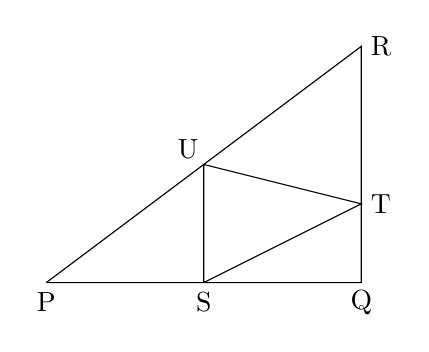
\begin{tikzpicture}
\draw (0,0) -- (4,0) -- (4,3) -- (0,0);
\draw (2,0) -- (4,1) -- (2,1.5) -- (2,0);
\node at (0,-0.25) {P};
\node at (2,-0.25) {S};
\node at (4,-0.25) {Q};
\node at (4.25,1) {T};
\node at (4.25,3) {R};
\node at (1.8,1.7) {U};
\end{tikzpicture}


\item Right triangle $PQR$ is to be constructed in the $xy-$plane so that the right angle is at $P$ and line $PR$ is parallel to the $x-$axis. The $x$ and $y$ coordinates of $P$, $Q$ and $R$ are to be integers that satisfy the inequalities: $-4\leq x\leq 5$ and $6\leq y\leq 16$. How many different triangles could be constructed with these properties?\hfill(2015)
\begin{multicols}{2}
\begin{enumerate}
\item $110$
\item $1,100$
\item $9,900$
\item $10,000$
\end{enumerate}
\end{multicols}


\item A coin is tossed thrice. Let $X$ be the event that head occurs in each of the first two tosses. Let $Y$ be the event that a tail occurs on the third toss. Let $Z$ be the event that two tails occur in three tosses. Based on the above information, which one of the following statements is TRUE?\hfill(2015)
\begin{multicols}{2}
\begin{enumerate}
\item $X$ and $Y$ are not independent
\item $Y$ and $Z$ are dependent
\item $Y$ and $Z$ are independent
\item $X$ and $Z$ are independent
\end{enumerate}
\end{multicols}


\item The partial differential equation $\frac{\partial u}{\partial t}+\frac{\partial\brak{\frac{u^{2}}{2}}}{\partial x}=0$ is\hfill(2015)
\begin{multicols}{2}
\begin{enumerate}
\item linear and first order
\item linear and second order
\item non-linear and first order
\item non-linear and second order
\end{enumerate}
\end{multicols}


\item The system of equations for the variables $x$ and $y$

$ax+by=e$

$cx+dy=f$

has a unique solution only if\hfill(2015)
\begin{multicols}{2}
\begin{enumerate}
\item $ad-bc\neq 0$
\item $ac-bd\neq 0$
\item $a+c\neq b+d$
\item $a-c\neq b-d$
\end{enumerate}
\end{multicols}


\item A linear mass-spring-dashpot system is over-damped. In free vibration, this system undergoes\hfill(2015)
\begin{multicols}{2}
\begin{enumerate}
\item non-oscillatory motion
\item random motion
\item oscillatory and periodic motion
\item oscillatory and non-periodic motion
\end{enumerate}
\end{multicols}